\documentclass[UTF8]{ctexart}
\usepackage[table]{xcolor}
\usepackage{algorithm}
\usepackage{algorithmic}
\usepackage{subfigure}
\usepackage{amsmath,bm}
\usepackage{fancybox}
\usepackage{listings}
\usepackage{xcolor}
\usepackage{diagbox}
\usepackage{amssymb}
\usepackage{amsmath}
\usepackage{amsthm}
\usepackage{empheq}
\usepackage{warpcol}
\usepackage{lscape}
\usepackage[framemethod=tikz]{mdframed}
\usepackage{mathtools}
\usepackage{fancyhdr} 
\usepackage{longtable,booktabs}                               
\usepackage{lastpage}                                           
\usepackage{layout} 


% 图表
\usepackage{array,multirow}
  \setlength\extrarowheight{2pt} % 行高增加
\usepackage{longtable}
\usepackage{graphicx}

\usepackage{listings}

\usepackage{xcolor}

	\definecolor{ocre}{RGB}{243,102,25}
	\definecolor{mygray}{RGB}{243,243,244}

%
%\lstset{
%columns=flexible,
%numbers=left,
%numberstyle=\footnotesize\color{darkgray}, 
%basicstyle=\small\ttfamily,
%stringstyle=\color{purple},
%keywordstyle=\color[RGB]{40,40,255}\bfseries,
%commentstyle=\it\color[RGB]{0,96,96},  
%stringstyle=\rmfamily\slshape\color[RGB]{128,0,0}, 
%showstringspaces=false,      
%% directivestyle=\color{blue},
%frame=shadowbox,
%%framerule=0pt,
%backgroundcolor=\color[RGB]{245,245,244},
%escapeinside=``, %逃逸字符(1左面的键),用于显示中文
%breaklines,
%extendedchars=false,
%%解决代码跨页时,章节标题,页眉等汉字不显示的问题
%xleftmargin=2em,xrightmargin=2em,
%aboveskip=1em,%设置边距
%tabsize=4, %设置tab空格数  
%showspaces=false %不显示空格 
%rulesepcolor=\color{red!20!green!20!blue!20}
%%rulesepcolor=\color{brown}
%}



% 行号
\usepackage{lineno}


% 引用
\usepackage[colorlinks=true,
            pdfborder=001,     
            citecolor=blue,
            linkcolor=red,
            anchorcolor=green,
            urlcolor=blue,
            bookmarksopen=true,bookmarksnumbered=true]{hyperref}
\usepackage{framed} 
\usepackage{ulem}
\usepackage{tabu}
\title{CS294A Lecture notes}
\author{Andrew Ng}
\begin{document}
\maketitle
\section{Introduction}
监督学习是人工智能最强大的工具之一,并由此产生了自动压缩编码识别,语音识别,自动驾驶汽车,以及不断提高对人类基因组的理解。 尽管取得了重大成就,今天的监督学习仍然受到严重限制。 具体来说,它的大多数应用程序仍然要求我们手动指定给算法的输入特征$x$。
一旦给出了一个好的特征表示,一个监督学习算法就可以做得很好。 但是在计算机视觉,音频处理和自然语言处理等领域,现在已经有数百甚至数千名研究人员花费了数年的时间,慢慢地辛苦地手工设计视觉,音频或文本特征。 虽然这个功能工程的大部分工作非常聪明,但我们不禁要问,是否我们能做得更好, 当然,这种劳动密集型的手动工作方法并不能很好地解决新问题。 此外,理想情况下,我们希望有一种算法能够自动学习比手动设计更好的特征表示。

这些课程描述了稀疏自动编码器学习算法,这是从未标记数据自动学习特征的一种方法。 在一些领域,如计算机视觉,这种方法本身并不是与最好的手动工作相竞争的,但是它所能学习的特性对于一系列问题(包括音频,文本等)是有用的。 此外,还有更复杂的稀疏自动编码器的版本(在这些笔记中没有描述,但是你会在后面听到更多的信息),这样做的确令人惊讶,而且在许多情况下,它们甚至比最好的手工表示更具竞争力或优越性。

这些课程的结构如下: 我们将首先描述前馈神经网络和监督学习的反向传播算法。 然后,我们展示了如何使用它来构造一个自动编码器,这是一个无监督的学习算法。 最后,我们基于此来衍生一个稀疏的自动编码器。 由于这些笔记用到了很多符号,最后一页将包含所用符号的摘要。

\section{Neural networks}
\subsection{Backpropagation algorithm}
假设我们有一个固定样本集 $ \{ (x^{(1)}, y^{(1)}), \ldots, (x^{(m)}, y^{(m)}) \}$,它包含 $ m $个样例。我们可以用批量梯度下降法来求解神经网络。具体来讲,对于单个样例 $ (x,y)$,其代价函数为:
\begin{align}
J(W,b; x,y) = \frac{1}{2} \left\| h_{W,b}(x) - y \right\|^2.
\nonumber \end{align}
这是一个(二分之一的)方差代价函数。给定一个包含 $ m $个样例的数据集,我们可以定义整体代价函数为:
\begin{align}
J(W,b)
&= \left[ \frac{1}{m} \sum_{i=1}^m J(W,b;x^{(i)},y^{(i)}) \right]
                       + \frac{\lambda}{2} \sum_{l=1}^{n_l-1} \; \sum_{i=1}^{s_l} \; \sum_{j=1}^{s_{l+1}} \left( W^{(l)}_{ji} \right)^2
 \nonumber \\
&= \left[ \frac{1}{m} \sum_{i=1}^m \left( \frac{1}{2} \left\| h_{W,b}(x^{(i)}) - y^{(i)} \right\|^2 \right) \right]
                       + \frac{\lambda}{2} \sum_{l=1}^{n_l-1} \; \sum_{i=1}^{s_l} \; \sum_{j=1}^{s_{l+1}} \left( W^{(l)}_{ji} \right)^2
\nonumber \end{align}
以上关于$ J(W,b)$定义中的第一项是一个均方差项。第二项是一个规则化项(也叫\textbf{权重衰减项}),其目的是减小权重的幅度,防止过度拟合.\footnote{注:通常权重衰减的计算并不使用偏置项 $ b^{(l)}_i$,比如我们在 $ J(W, b)$ 的定义中就没有使用。一般来说,将偏置项包含在权重衰减项中只会对最终的神经网络产生很小的影响。如果你在斯坦福选修过CS229(机器学习)课程,或者在YouTube上看过课程视频,你会发现这个权重衰减实际上是课上提到的贝叶斯规则化方法的变种。在贝叶斯规则化方法中,我们将高斯先验概率引入到参数中计算MAP(极大后验)估计(而不是极大似然估计)。}

权重衰减参数 $ \lambda $用于控制公式中两项的相对重要性。在此重申一下这两个复杂函数的含义:$ J(W,b;x,y)$ 是针对单个样例计算得到的方差代价函数;$ J(W,b)$ 是整体样本代价函数,它包含权重衰减项。

以上的代价函数经常被用于分类和回归问题。在分类问题中,我们用 $ y = 0 or  1$ 代表两种类型的标签(回想一下,这是因为 sigmoid激活函数的值域为 $ [0,1]$;如果我们使用双曲正切型激活函数,那么应该选用 $ -1$ 和 $ +1$ 作为标签)。对于回归问题,我们首先要变换输出值域(译者注:也就是 $ y$),以保证其范围为 $ [0,1]$ (同样地,如果我们使用双曲正切型激活函数,要使输出值域为 $ [-1,1]$)。

我们的目标是针对参数 $ W$ 和 $ b $来求其函数 $ J(W,b) $的最小值。为了求解神经网络,我们需要将每一个参数 $ W^{(l)}_{ij}$ 和 $ b^{(l)}_i$ 初始化为一个很小的、接近零的随机值(比如说,使用正态分布 $ {Normal}(0,\epsilon^2) $生成的随机值,其中 $ \epsilon $设置为 $ 0.01$ ),之后对目标函数使用诸如批量梯度下降法的最优化算法。因为 $ J(W, b)$ 是一个非凸函数,梯度下降法很可能会收敛到局部最优解;但是在实际应用中,梯度下降法通常能得到令人满意的结果。最后,需要再次强调的是,要将参数进行随机初始化,而不是全部置为 $ 0$。如果所有参数都用相同的值作为初始值,那么所有隐藏层单元最终会得到与输入值有关的、相同的函数(也就是说,对于所有 $ i$,$ W^{(1)}_{ij}$都会取相同的值,那么对于任何输入 $ x$ 都会有:$ a^{(2)}_1 = a^{(2)}_2 = a^{(2)}_3 = \ldots $)。随机初始化的目的是使\textbf{对称失效}。

梯度下降法中每一次迭代都按照如下公式对参数 $ W$ 和$ b $进行更新:
\begin{align}
W_{ij}^{(l)} &= W_{ij}^{(l)} - \alpha \frac{\partial}{\partial W_{ij}^{(l)}} J(W,b) \nonumber \\
b_{i}^{(l)} &= b_{i}^{(l)} - \alpha \frac{\partial}{\partial b_{i}^{(l)}} J(W,b)
\nonumber \end{align}
其中 $ \alpha $是学习速率。其中关键步骤是计算偏导数。我们现在来讲一下\textbf{反向传播算法},它是计算偏导数的一种有效方法。

我们首先来讲一下如何使用反向传播算法来计算 $ \frac{\partial}{\partial W_{ij}^{(l)}} J(W,b; x, y) $和  $ \frac{\partial}{\partial b_{i}^{(l)}} J(W,b; x, y)$,这两项是单个样例 $ (x,y) $的代价函数 $ J(W,b;x,y) $的偏导数。一旦我们求出该偏导数,就可以推导出整体代价函数 $ J(W,b)$ 的偏导数:
\begin{align}
\frac{\partial}{\partial W_{ij}^{(l)}} J(W,b) &=
\left[ \frac{1}{m} \sum_{i=1}^m \frac{\partial}{\partial W_{ij}^{(l)}} J(W,b; x^{(i)}, y^{(i)}) \right] + \lambda W_{ij}^{(l)} \nonumber \\
\frac{\partial}{\partial b_{i}^{(l)}} J(W,b) &=
\frac{1}{m}\sum_{i=1}^m \frac{\partial}{\partial b_{i}^{(l)}} J(W,b; x^{(i)}, y^{(i)})
\nonumber \end{align}
以上两行公式稍有不同,第一行比第二行多出一项,是因为权重衰减是作用于 $ W $而不是 $ b$.

反向传播算法的思路如下:给定一个样例 $ (x,y)$,我们首先进行“前向传导”运算,计算出网络中所有的激活值,包括 $ h_{W,b}(x)$ 的输出值。之后,针对第 $ l$ 层的每一个节点 $ i$,我们计算出其“残差” $ \delta^{(l)}_i$,该残差表明了该节点对最终输出值的残差产生了多少影响。对于最终的输出节点,我们可以直接算出网络产生的激活值与实际值之间的差距,我们将这个差距定义为 $ \delta^{(n_l)}_i $(第 $ n_l$ 层表示输出层)。对于隐藏单元我们如何处理呢?我们将基于节点(译者注:第 $ l+1$ 层节点)残差的加权平均值计算 $ \delta^{(l)}_i$,这些节点以 $ a^{(l)}_i $作为输入。下面将给出反向传导算法的细节:
\begin{enumerate}
\item
进行前馈传导计算,利用前向传导公式,得到 $ L_2, L_3, \ldots $ 直到输出层 $ L_{n_l} $的激活值。
\item
对于第 $ n_l$ 层(输出层)的每个输出单元 $ i$,我们根据以下公式计算残差:
\begin{align}
\delta^{(n_l)}_i
= \frac{\partial}{\partial z^{(n_l)}_i} \;\;
        \frac{1}{2} \left\|y - h_{W,b}(x)\right\|^2 = - (y_i - a^{(n_l)}_i) \cdot f'(z^{(n_l)}_i)
\nonumber \end{align}
%[译者注:
%\begin{align}
%\delta^{(n_l)}_i &= \frac{\partial}{\partial z^{n_l}_i}J(W,b;x,y)
% = \frac{\partial}{\partial z^{n_l}_i}\frac{1}{2} \left\|y - h_{W,b}(x)\right\|^2 \nonumber \\
% &= \frac{\partial}{\partial z^{n_l}_i}\frac{1}{2} \sum_{j=1}^{S_{n_l}} (y_j-a_j^{(n_l)})^2
% = \frac{\partial}{\partial z^{n_l}_i}\frac{1}{2} \sum_{j=1}^{S_{n_l}} (y_j-f(z_j^{(n_l)}))^2 \nonumber \\
% &= - (y_i - f(z_i^{(n_l)})) \cdot f'(z^{(n_l)}_i)
% = - (y_i - a^{(n_l)}_i) \cdot f'(z^{(n_l)}_i)
%\nonumber \end{align}
%]
\item
对 $ l = n_l-1, n_l-2, n_l-3, \ldots, 2 $的各个层,第 $ l $层的第 $ i$ 个节点的残差计算方法如下:
 
\[\delta^{(l)}_i = \left( \sum_{j=1}^{s_{l+1}} W^{(l)}_{ji} \delta^{(l+1)}_j \right) f'(z^{(l)}_i)\]
%[译者注:
%\begin{align}
%\delta^{(n_l-1)}_i &=\frac{\partial}{\partial z^{n_l-1}_i}J(W,b;x,y)
% = \frac{\partial}{\partial z^{n_l-1}_i}\frac{1}{2} \left\|y - h_{W,b}(x)\right\|^2 
% = \frac{\partial}{\partial z^{n_l-1}_i}\frac{1}{2} \sum_{j=1}^{S_{n_l}}(y_j-a_j^{(n_l)})^2 \nonumber \\
%&= \frac{1}{2} \sum_{j=1}^{S_{n_l}}\frac{\partial}{\partial z^{n_l-1}_i}(y_j-a_j^{(n_l)})^2
% = \frac{1}{2} \sum_{j=1}^{S_{n_l}}\frac{\partial}{\partial z^{n_l-1}_i}(y_j-f(z_j^{(n_l)}))^2 \nonumber \\
%&= \sum_{j=1}^{S_{n_l}}-(y_j-f(z_j^{(n_l)})) \cdot \frac{\partial}{\partial z_i^{(n_l-1)}}f(z_j^{(n_l)})
% = \sum_{j=1}^{S_{n_l}}-(y_j-f(z_j^{(n_l)})) \cdot  f'(z_j^{(n_l)}) \cdot \frac{\partial z_j^{(n_l)}}{\partial z_i^{(n_l-1)}} \nonumber \\
%&= \sum_{j=1}^{S_{n_l}} \delta_j^{(n_l)} \cdot \frac{\partial z_j^{(n_l)}}{\partial z_i^{n_l-1}}
% = \sum_{j=1}^{S_{n_l}} \left(\delta_j^{(n_l)} \cdot \frac{\partial}{\partial z_i^{n_l-1}}\sum_{k=1}^{S_{n_l-1}}f(z_k^{n_l-1}) \cdot W_{jk}^{n_l-1}\right) \nonumber \\
%&= \sum_{j=1}^{S_{n_l}} \delta_j^{(n_l)} \cdot  W_{ji}^{n_l-1} \cdot f'(z_i^{n_l-1})
% = \left(\sum_{j=1}^{S_{n_l}}W_{ji}^{n_l-1}\delta_j^{(n_l)}\right)f'(z_i^{n_l-1})
%\nonumber \end{align}
%将上式中的$ n_l-1$与$ n_l$的关系替换为$ l$与$ l+1$的关系,就可以得到:
%\[\delta^{(l)}_i = \left( \sum_{j=1}^{s_{l+1}} W^{(l)}_{ji} \delta^{(l+1)}_j \right) f'(z^{(l)}_i)\]
%以上逐次从后向前求导的过程即为“反向传导”的本意所在。 ]
\item
计算我们需要的偏导数,计算方法如下:
\begin{align}
\frac{\partial}{\partial W_{ij}^{(l)}} J(W,b; x, y) &= a^{(l)}_j \delta_i^{(l+1)} \nonumber \\
\frac{\partial}{\partial b_{i}^{(l)}} J(W,b; x, y) &= \delta_i^{(l+1)}.
\nonumber \end{align}
\end{enumerate}

最后,我们用矩阵-向量表示法重写以上算法。我们使用“$ \bullet$” 表示向量乘积运算符(在Matlab或Octave里用“.*”表示,也称作阿达马乘积)。若 $ a = b \bullet c$,则 $ a_i = b_ic_i$。在上一个教程中我们扩展了 $ f(\cdot) $的定义,使其包含向量运算,这里我们也对偏导数 $ f'(\cdot)$ 也做了同样的处理(于是又有  $ f'([z_1, z_2, z_3]) = [f'(z_1), f'(z_2), f'(z_3)] $)。

那么,反向传播算法可表示为以下几个步骤:
\begin{enumerate}
\item
进行前馈传导计算,利用前向传导公式,得到 $ L_2, L_3, \ldots$直到输出层 $ L_{n_l}$ 的激活值。
\item
对输出层(第 $ n_l$ 层),计算:
 \begin{align}
\delta^{(n_l)}
= - (y - a^{(n_l)}) \bullet f'(z^{(n_l)})
\nonumber \end{align}
\item
对于 $ l = n_l-1, n_l-2, n_l-3, \ldots, 2 $的各层,计算:
 \begin{align}
\delta^{(l)} = \left((W^{(l)})^T \delta^{(l+1)}\right) \bullet f'(z^{(l)})
\nonumber \end{align}
\item
计算最终需要的偏导数值:
 \begin{align}
\nabla_{W^{(l)}} J(W,b;x,y) &= \delta^{(l+1)} (a^{(l)})^T, \nonumber \\
\nabla_{b^{(l)}} J(W,b;x,y) &= \delta^{(l+1)}.
\nonumber \end{align}
\end{enumerate}
\textbf{实现中应注意}:在以上的第2步和第3步中,我们需要为每一个 $ i $值计算其 $ f'(z^{(l)}_i)$。假设 $ f(z) $是sigmoid函数,并且我们已经在前向传导运算中得到了 $ a^{(l)}_i$。那么,使用我们早先推导出的 $ f'(z)$表达式,就可以计算得到 $ f'(z^{(l)}_i) = a^{(l)}_i (1- a^{(l)}_i)$。

最后,我们将对梯度下降算法做个全面总结。在下面的伪代码中,$ \Delta W^{(l)}$ 是一个与矩阵 $ W^{(l)}$ 维度相同的矩阵,$ \Delta b^{(l)}$ 是一个与 $ b^{(l)} $维度相同的向量。注意这里“$ \Delta W^{(l)}$”是一个矩阵,而不是“$ \Delta $与 $ W^{(l)} $相乘”。下面,我们实现批量梯度下降法中的一次迭代:
\begin{enumerate}
\item
对于所有 $ l$,令 $ \Delta W^{(l)} := 0 $,  $ \Delta b^{(l)} := 0 $(设置为全零矩阵或全零向量)
\item
对于 $ i = 1$ 到 $ m$,
\begin{enumerate}
\item 使用反向传播算法计算 $ \nabla_{W^{(l)}} J(W,b;x,y) $和 $ \nabla_{b^{(l)}} J(W,b;x,y)$.
\item 计算 $ \Delta W^{(l)} := \Delta W^{(l)} + \nabla_{W^{(l)}} J(W,b;x,y)$
\item 计算 $ \Delta b^{(l)} := \Delta b^{(l)} + \nabla_{b^{(l)}} J(W,b;x,y)$
\end{enumerate}
\item 更新权重参数:
 \begin{align}
W^{(l)} &= W^{(l)} - \alpha \left[ \left(\frac{1}{m} \Delta W^{(l)} \right) + \lambda W^{(l)}\right] \nonumber \\
b^{(l)} &= b^{(l)} - \alpha \left[\frac{1}{m} \Delta b^{(l)}\right]
\nonumber \end{align}
\end{enumerate}
现在,我们可以重复梯度下降法的迭代步骤来减小代价函数 $ J(W,b)$ 的值,进而求解我们的神经网络。


\subsection{Gradient checking and advanced optimization}
众所周知,反向传播算法很难调试得到正确结果,尤其是当实现程序存在很多难于发现的bug时。举例来说,索引的缺位错误(off-by-one error)会导致只有部分层的权重得到训练,再比如忘记计算偏置项。这些错误会使你得到一个看似十分合理的结果(但实际上比正确代码的结果要差)。因此,但从计算结果上来看,我们很难发现代码中有什么东西遗漏了。本节中,我们将介绍一种对求导结果进行数值检验的方法,该方法可以验证求导代码是否正确。另外,使用本节所述求导检验方法,可以帮助你提升写正确代码的信心。

缺位错误(Off-by-one error)举例说明:比如  for 循环中循环 $ m$次,正确应该是  $for (i=1;i<=m;~i++)$,但有时程序员疏忽,会写成  $for (i=1;i<m;i++)$,这就是缺位错误。

假设我们想要最小化以 $ \theta $为自变量的目标函数$ J(\theta)$。假设 $ J : \Re \mapsto \Re$,则 $ \theta \in \Re$。在一维的情况下,一次迭代的梯度下降公式是
\begin{align}
\theta := \theta - \alpha \frac{d}{d\theta}J(\theta).
\nonumber \end{align}

再假设我们已经用代码实现了计算 $ \frac{d}{d\theta}J(\theta) $的函数 $ g(\theta)$,接着我们使用  $ \theta := \theta - \alpha g(\theta)$ 来实现梯度下降算法。那么我们如何检验 $ g $的实现是否正确呢?
回忆导数的数学定义:
\begin{align}
\frac{d}{d\theta}J(\theta) = \lim_{\epsilon \rightarrow 0}
\frac{J(\theta+ \epsilon) - J(\theta-\epsilon)}{2 \epsilon}.
\nonumber \end{align}
那么对于任意 $ \theta$ 值,我们都可以对等式左边的导数用:
\begin{align}
\frac{J(\theta+{\rm EPSILON}) - J(\theta-{\rm EPSILON})}{2 \times {\rm EPSILON}}
\nonumber \end{align}
来近似。

实际应用中,我们常将 EPSILON 设为一个很小的常量,比如在$ 10^{-4} $数量级(虽然 $ EPSILON $的取值范围可以很大,但是我们不会将它设得太小,比如 $ 10^{-20}$,因为那将导致数值舍入误差。)

给定一个被认为能计算 $ \frac{d}{d\theta}J(\theta) $的函数$ g(\theta)$,我们可以用下面的数值检验公式
\begin{align}
g(\theta) \approx
\frac{J(\theta+{\rm EPSILON}) - J(\theta-{\rm EPSILON})}{2 \times {\rm EPSILON}}.
\nonumber \end{align}
计算两端是否一样来检验函数是否正确。

上式两端值的接近程度取决于 $ J$ 的具体形式。但是在假定$ {\rm EPSILON} = 10^{-4} $的情况下,你通常会发现上式左右两端至少有4位有效数字是一样的(通常会更多)。

现在,考虑 $ \theta \in \Re^n$ 是一个向量而非一个实数(那么就有$ n$个参数要学习得到),并且 $ J: \Re^n \mapsto \Re$。在神经网络的例子里我们使用 $ J(W,b)$,可以想象为把参数 $ W,b$ 组合扩展成一个长向量 $ \theta$。现在我们将求导检验方法推广到一般化,即 $ \theta $是一个向量的情况。
假设我们有一个用于计算 $ \frac{\partial}{\partial \theta_i} J(\theta)$的函数 $ g_i(\theta)$;我们想要检验 $ g_i $是否输出正确的求导结果。我们定义 $ \theta^{(i+)} = \theta +
{\rm EPSILON} \times \vec{e}_i$,其中
\begin{align}
\vec{e}_i = \begin{bmatrix}0 \nonumber \\ 0 \nonumber \\ \vdots \nonumber \\ 1 \nonumber \\ \vdots \nonumber \\ 0\end{bmatrix}
\nonumber \end{align}
是第 $ i$ 个基向量(维度和 $ \theta $相同,在第 $ i $行是“$ 1$”而其他行是“$ 0$”)。所以,$ \theta^{(i+)}$ 和 $ \theta$ 几乎相同,除了第 $ i $行元素增加了 EPSILON。类似地,$ \theta^{(i-)} = \theta - {\rm EPSILON} \times \vec{e}_i $得到的第 $ i $行减小了 EPSILON。然后我们可以对每个 $ i $检查下式是否成立,进而验证 $ g_i(\theta) $的正确性:
\begin{align}
g_i(\theta) \approx
\frac{J(\theta^{(i+)}) - J(\theta^{(i-)})}{2 \times {\rm EPSILON}}.
\nonumber \end{align}

当用反射传播算法求解神经网络时,正确算法实现会得到:
\begin{align}
\nabla_{W^{(l)}} J(W,b) &= \left( \frac{1}{m} \Delta W^{(l)} \right) + \lambda W^{(l)} \nonumber \\
\nabla_{b^{(l)}} J(W,b) &= \frac{1}{m} \Delta b^{(l)}.
\nonumber \end{align}

以上结果与反向传播算法中的最后一段伪代码一致,都是计算梯度下降。为了验证梯度下降代码的正确性,使用上述数值检验方法计算 $ J(W,b) $的导数,然后验证 $ \left(\frac{1}{m}\Delta W^{(l)} \right) + \lambda W$ 与 $ \frac{1}{m}\Delta b^{(l)} $是否能够给出正确的求导结果。

迄今为止,我们的讨论都集中在使用梯度下降法来最小化 $ J(\theta)$。如果你已经实现了一个计算 $ J(\theta)$ 和 $ \nabla_\theta J(\theta) $的函数,那么其实还有更精妙的算法来最小化 $ J(\theta)$。举例来说,可以想象这样一个算法:它使用梯度下降,并能够自动调整学习速率 $ \alpha$,以得到合适的步长值,最终使 $ \theta$ 能够快速收敛到一个局部最优解。还有更妙的算法:比如可以寻找一个Hessian矩阵的近似,得到最佳步长值,使用该步长值能够更快地收敛到局部最优(和牛顿法类似)。此类算法的详细讨论已超出了这份讲义的范围,但是L-BFGS算法我们以后会有论述(另一个例子是共轭梯度算法)。你将在编程练习里使用这些算法中的一个。使用这些高级优化算法时,你需要提供关键的函数:即对于任一个 $ \theta$,需要你计算出 $ J(\theta)$ 和 $ \nabla_\theta J(\theta)$。之后,这些优化算法会自动调整学习速率/步长值  $ \alpha $的大小(并计算Hessian近似矩阵等等)来自动寻找 $ J(\theta)$ 最小化时$ \theta$ 的值。诸如L-BFGS和共轭梯度算法通常比梯度下降法快很多。
\section{Autoencoders and sparsity}
目前为止,我们已经讨论了神经网络在有监督学习中的应用。在有监督学习中,训练样本是有类别标签的。现在假设我们只有一个没有带类别标签的训练样本集合 $\{x^{(1)}, x^{(2)}, x^{(3)}, \ldots\}$ ,其中 $x^{(i)} \in \Re^{n} $。自编码神经网络是一种无监督学习算法,它使用了反向传播算法,并让目标值等于输入值,比如 $ y^{(i)} = x^{(i)} $。下图是一个自编码神经网络的示例。

\begin{figure}[H]
\centering
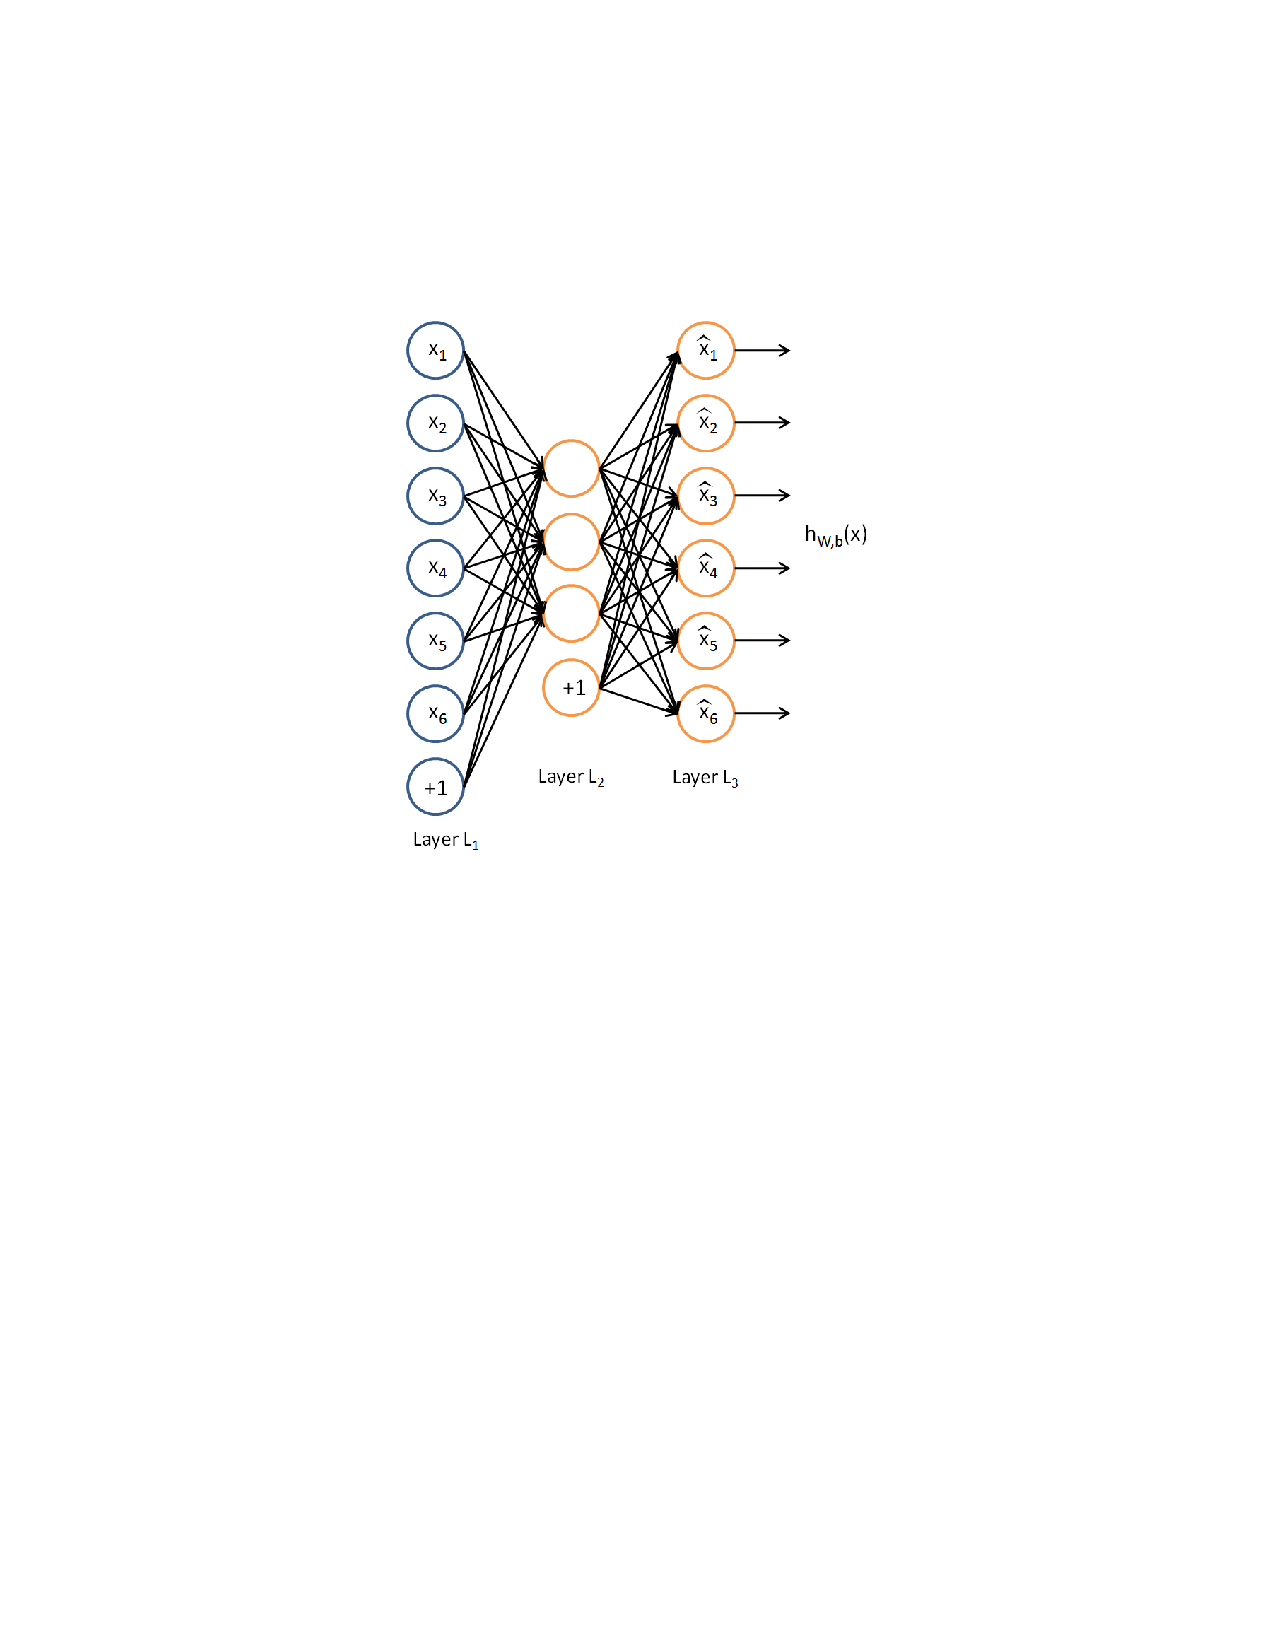
\includegraphics[width=8cm]{fig/1_1.pdf}
\end{figure}

自编码神经网络尝试学习一个 $ h_{W,b}(x) \approx x $的函数。换句话说,它尝试逼近一个恒等函数,从而使得输出 $ \hat{x} $接近于输入 $ x$ 。恒等函数虽然看上去不太有学习的意义,但是当我们为自编码神经网络加入某些限制,比如限定隐藏神经元的数量,我们就可以从输入数据中发现一些有趣的结构。举例来说,假设某个自编码神经网络的输入 $ x $ 是一张 $ 10 \times 10$ 图像(共100个像素)的像素灰度值,于是 $ n=100$ ,其隐藏层 $ L_2 $中有50个隐藏神经元。注意,输出也是100维的 $ y \in \Re^{100}$ 。由于只有50个隐藏神经元,我们迫使自编码神经网络去学习输入数据的压缩表示,也就是说,它必须从50维的隐藏神经元激活度向量 $ a^{(2)} \in \Re^{50} $中\textbf{重构}出100维的像素灰度值输入 $ x$ 。如果网络的输入数据是完全随机的,比如每一个输入 $ x_i $都是一个跟其它特征完全无关的独立同分布高斯随机变量,那么这一压缩表示将会非常难学习。但是如果输入数据中隐含着一些特定的结构,比如某些输入特征是彼此相关的,那么这一算法就可以发现输入数据中的这些相关性。\footnote{事实上,这一简单的自编码神经网络通常可以学习出一个跟主元分析(PCA)结果非常相似的输入数据的低维表示。}

我们刚才的论述是基于隐藏神经元数量较小的假设。但是即使隐藏神经元的数量较大(可能比输入像素的个数还要多),我们仍然通过给自编码神经网络施加一些其他的限制条件来发现输入数据中的结构。具体来说,如果我们给隐藏神经元加入\textbf{稀疏性限制},那么自编码神经网络即使在隐藏神经元数量较多的情况下仍然可以发现输入数据中一些有趣的结构。

稀疏性可以被简单地解释如下。如果当神经元的输出接近于1的时候我们认为它被激活,而输出接近于0的时候认为它被抑制,那么使得神经元大部分的时间都是被抑制的限制则被称作稀疏性限制。\footnote{这里我们假设的神经元的激活函数是sigmoid函数。如果你使用tanh作为激活函数的话,当神经元输出为-1的时候,我们认为神经元是被抑制的.}

注意到 $ a^{(2)}_j $表示隐藏神经元 $ j $的激活度,但是这一表示方法中并未明确指出哪一个输入 $ x $带来了这一激活度。所以我们将使用 $ a^{(2)}_j(x) $来表示在给定输入为 $ x $情况下,自编码神经网络隐藏神经元 $ j $的激活度。 进一步,让
\begin{align}
\hat\rho_j = \frac{1}{m} \sum_{i=1}^m \left[ a^{(2)}_j(x^{(i)}) \right]
\nonumber \end{align}

表示隐藏神经元 $ j $的平均活跃度(在训练集上取平均)。我们可以近似的加入一条限制
\begin{align}
\hat\rho_j = \rho,
\nonumber \end{align}
其中, $ \rho $是\textbf{稀疏性参数},通常是一个接近于0的较小的值(比如 $ \rho = 0.05 $)。换句话说,我们想要让隐藏神经元 $ j $的平均活跃度接近0.05。为了满足这一条件,隐藏神经元的活跃度必须接近于0。
为了实现这一限制,我们将会在我们的优化目标函数中加入一个额外的惩罚因子,而这一惩罚因子将惩罚那些 $ \hat\rho_j $和 $ \rho $有显著不同的情况从而使得隐藏神经元的平均活跃度保持在较小范围内。惩罚因子的具体形式有很多种合理的选择,我们将会选择以下这一种:
\begin{align}
\sum_{j=1}^{s_2} \rho \log \frac{\rho}{\hat\rho_j} + (1-\rho) \log \frac{1-\rho}{1-\hat\rho_j}.
\nonumber \end{align}
这里, $ s_2 $是隐藏层中隐藏神经元的数量,而索引 $ j $依次代表隐藏层中的每一个神经元。如果你对相对熵(KL divergence)比较熟悉,这一惩罚因子实际上是基于它的。于是惩罚因子也可以被表示为
\begin{align}
\sum_{j=1}^{s_2} {\rm KL}(\rho || \hat\rho_j),
\nonumber \end{align}
其中 $ {\rm KL}(\rho || \hat\rho_j)
 = \rho \log \frac{\rho}{\hat\rho_j} + (1-\rho) \log \frac{1-\rho}{1-\hat\rho_j}$  是一个以 $ \rho$ 为均值和一个以 $ \hat\rho_j $为均值的两个伯努利随机变量之间的相对熵。相对熵是一种标准的用来测量两个分布之间差异的方法。(如果你没有见过相对熵,不用担心,所有你需要知道的内容都会被包含在这份笔记之中。)

这一惩罚因子有如下性质,当 $ \hat\rho_j = \rho $时 $ {\rm KL}(\rho || \hat\rho_j) = 0$ ,并且随着 $ \hat\rho_j $ 与 $ \rho$ 之间的差异增大而单调递增。举例来说,在下图中,我们设定 $ \rho = 0.2$ 并且画出了相对熵值 $ {\rm KL}(\rho || \hat\rho_j)$ 随着 $ \hat\rho_j $变化的变化。

\begin{figure}[H]
\centering
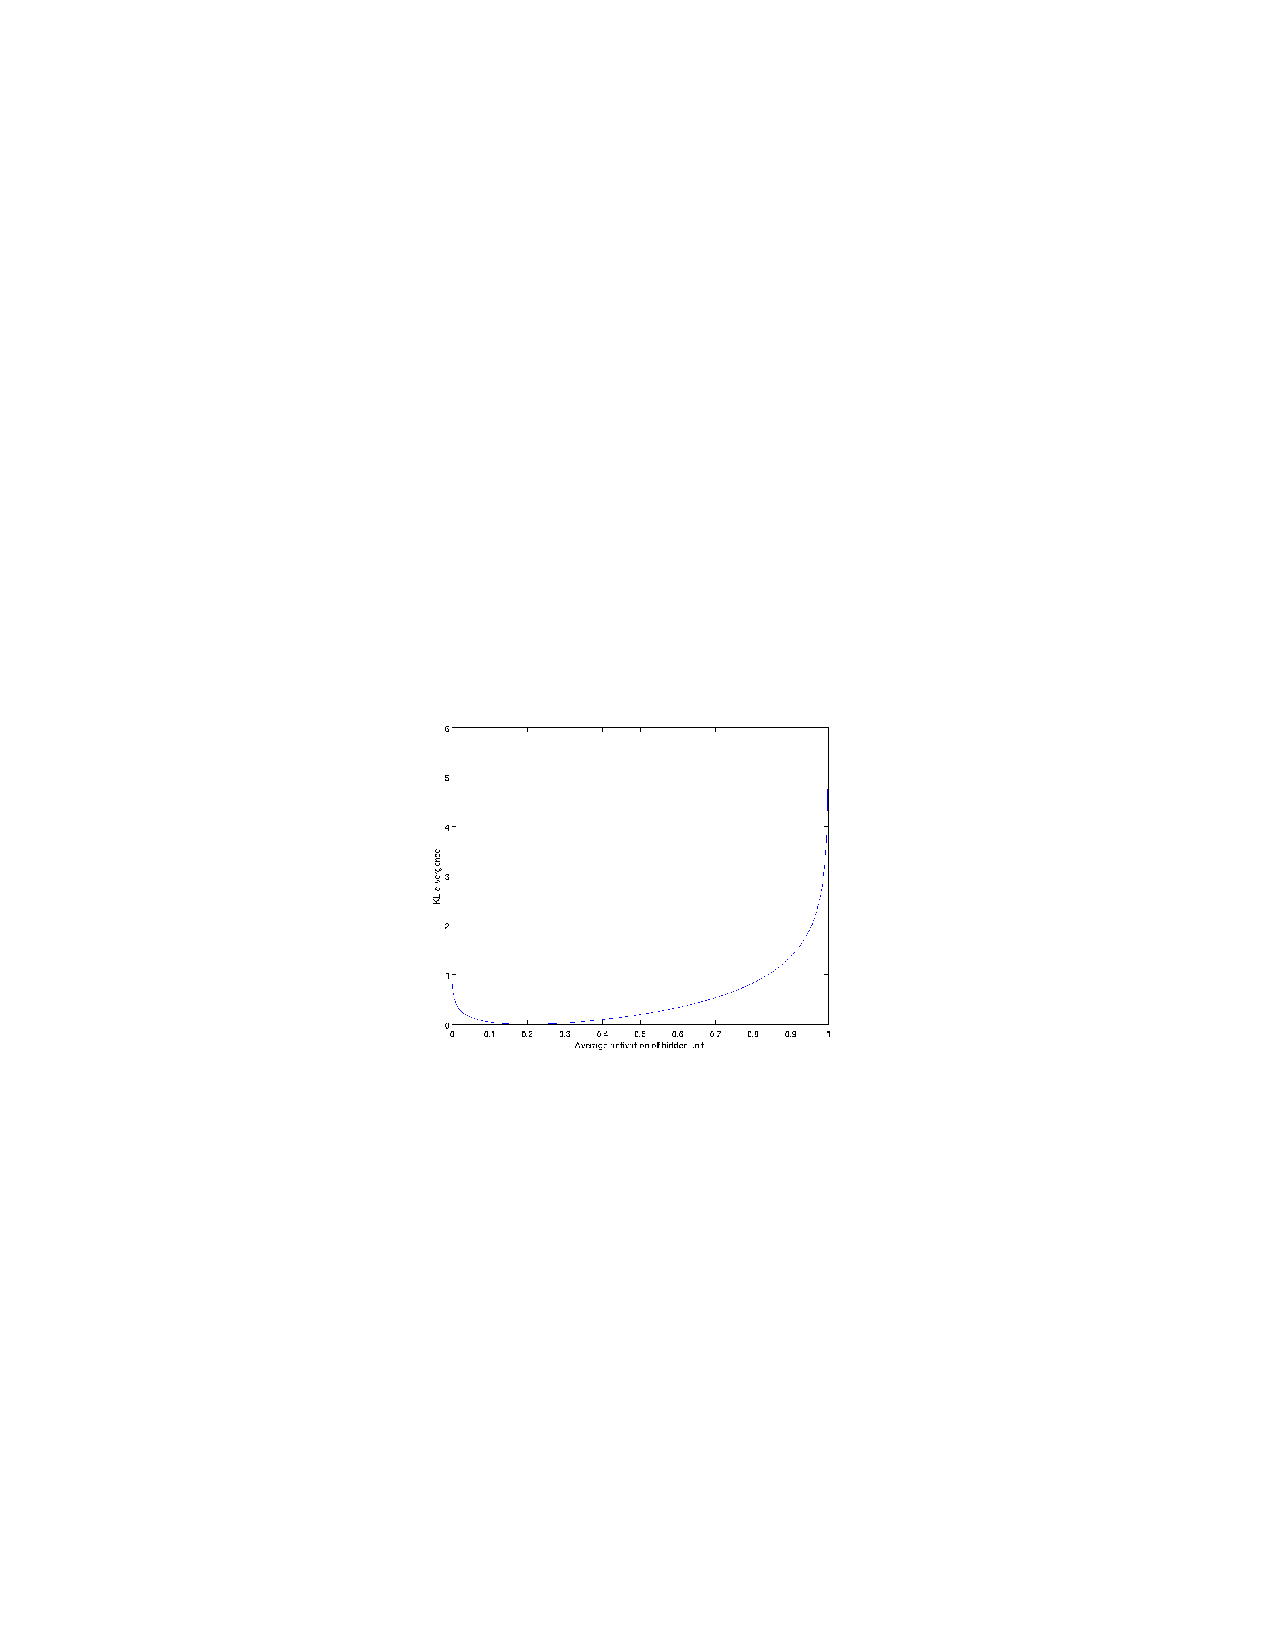
\includegraphics[width=8cm]{fig/1_2.pdf}
\end{figure}

我们可以看出,相对熵在 $ \hat\rho_j = \rho$  时达到它的最小值0,而当 $ \hat\rho_j $ 靠近0或者1的时候,相对熵则变得非常大(其实是趋向于$ \infty$ )。所以,最小化这一惩罚因子具有使得 $ \hat\rho_j$  靠近 $ \rho $ 的效果。 现在,我们的总体代价函数可以表示为
\begin{align}
J_{\rm sparse}(W,b) = J(W,b) + \beta \sum_{j=1}^{s_2} {\rm KL}(\rho || \hat\rho_j),
\nonumber \end{align}
其中 $ J(W,b) $ 如之前所定义,而 $ \beta $ 控制稀疏性惩罚因子的权重。 $ \hat\rho_j $ 项则也(间接地)取决于 $ W,b$  ,因为它是隐藏神经元 $ j $ 的平均激活度,而隐藏层神经元的激活度取决于 $ W,b $ 。

为了对相对熵进行导数计算,我们可以使用一个易于实现的技巧,这只需要在你的程序中稍作改动即可。具体来说,前面在后向传播算法中计算第二层( $ l=2$  )更新的时候我们已经计算了
\begin{align}
\delta^{(2)}_i = \left( \sum_{j=1}^{s_{2}} W^{(2)}_{ji} \delta^{(3)}_j \right) f'(z^{(2)}_i),
\nonumber \end{align}
现在我们将其换成
\begin{align}
\delta^{(2)}_i =
  \left( \left( \sum_{j=1}^{s_{2}} W^{(2)}_{ji} \delta^{(3)}_j \right)
+ \beta \left( - \frac{\rho}{\hat\rho_i} + \frac{1-\rho}{1-\hat\rho_i} \right) \right) f'(z^{(2)}_i) .
\nonumber \end{align}
就可以了。

有一个需要注意的地方就是我们需要知道 $ \hat\rho_i $ 来计算这一项更新。所以在计算任何神经元的后向传播之前,你需要对所有的训练样本计算一遍前向传播,从而获取平均激活度。如果你的训练样本可以小到被整个存到内存之中(对于编程作业来说,通常如此),你可以方便地在你所有的样本上计算前向传播并将得到的激活度存入内存并且计算平均激活度 。然后你就可以使用事先计算好的激活度来对所有的训练样本进行后向传播的计算。如果你的数据量太大,无法全部存入内存,你就可以扫过你的训练样本并计算一次前向传播,然后将获得的结果累积起来并计算平均激活度 $ \hat\rho_i $ (当某一个前向传播的结果中的激活度 $ a^{(2)}_i$  被用于计算平均激活度 $ \hat\rho_i$  之后就可以将此结果删除)。然后当你完成平均激活度 $ \hat\rho_i$  的计算之后,你需要重新对每一个训练样本做一次前向传播从而可以对其进行后向传播的计算。对于后一种情况,你对每一个训练样本需要计算两次前向传播,所以在计算上的效率会稍低一些。
证明上面算法能达到梯度下降效果的完整推导过程不再本教程的范围之内。不过如果你想要使用经过以上修改的后向传播来实现自编码神经网络,那么你就会对目标函数 $ J_{\rm sparse}(W,b)$  做梯度下降。使用梯度验证方法,你可以自己来验证梯度下降算法是否正确。

\section{Visualization}
训练完(稀疏)自编码器,我们还想把这自编码器学到的函数可视化出来,好弄明白它到底学到了什么。我们以在$10\times10$图像(即$n=100$)上训练自编码器为例。在该自编码器中,每个隐藏单元$i$对如下关于输入的函数进行计算:
\begin{align}
a^{(2)}_i = f\left(\sum_{j=1}^{100} W^{(1)}_{ij} x_j  + b^{(1)}_i \right).
\nonumber \end{align}
我们将要可视化的函数,就是上面这个以2D图像为输入、并由隐藏单元i计算出来的函数。它是依赖于参数$ W^{(1)}_{ij}$ 的(暂时忽略偏置项$b_i$)。需要注意的是,$ a^{(2)}_i$ 可看作输入$ x$ 的非线性特征。不过还有个问题:什么样的输入图像$ x$ 可让$ a^{(2)}_i$ 得到最大程度的激励?(通俗一点说,隐藏单元$ i$ 要找个什么样的特征?)。这里我们必须给$ x$ 加约束,否则会得到平凡解。若假设输入有范数约束$ ||x||^2 = \sum_{i=1}^{100} x_i^2 \leq 1$ ,则可证(请读者自行推导)令隐藏单元$ i$ 得到最大激励的输入应由下面公式计算的像素$ x_j$ 给出(共需计算100个像素,$j=1,\cdots,100$):
\begin{align}
x_j = \frac{W^{(1)}_{ij}}{\sqrt{\sum_{j=1}^{100} (W^{(1)}_{ij})^2}}.
\nonumber \end{align}
当我们用上式算出各像素的值、把它们组成一幅图像、并将图像呈现在我们面前之时,隐藏单元$ i$ 所追寻特征的真正含义也渐渐明朗起来。
假如我们训练的自编码器有100个隐藏单元,可视化结果就会包含100幅这样的图像——每个隐藏单元都对应一幅图像。审视这100幅图像,我们可以试着体会这些隐藏单元学出来的整体效果是什么样的。

当我们对稀疏自编码器(100个隐藏单元,在$10\times 10$像素\footnote{下面的结果是通过训练\textbf{被白化}的自然图像获得的。美白是预处理步骤,通过使相邻像素变得较少相关来消除输入中的冗余.}的输入上训练 )进行上述可视化处理之后,结果如下所示:

\begin{figure}[H]
\centering
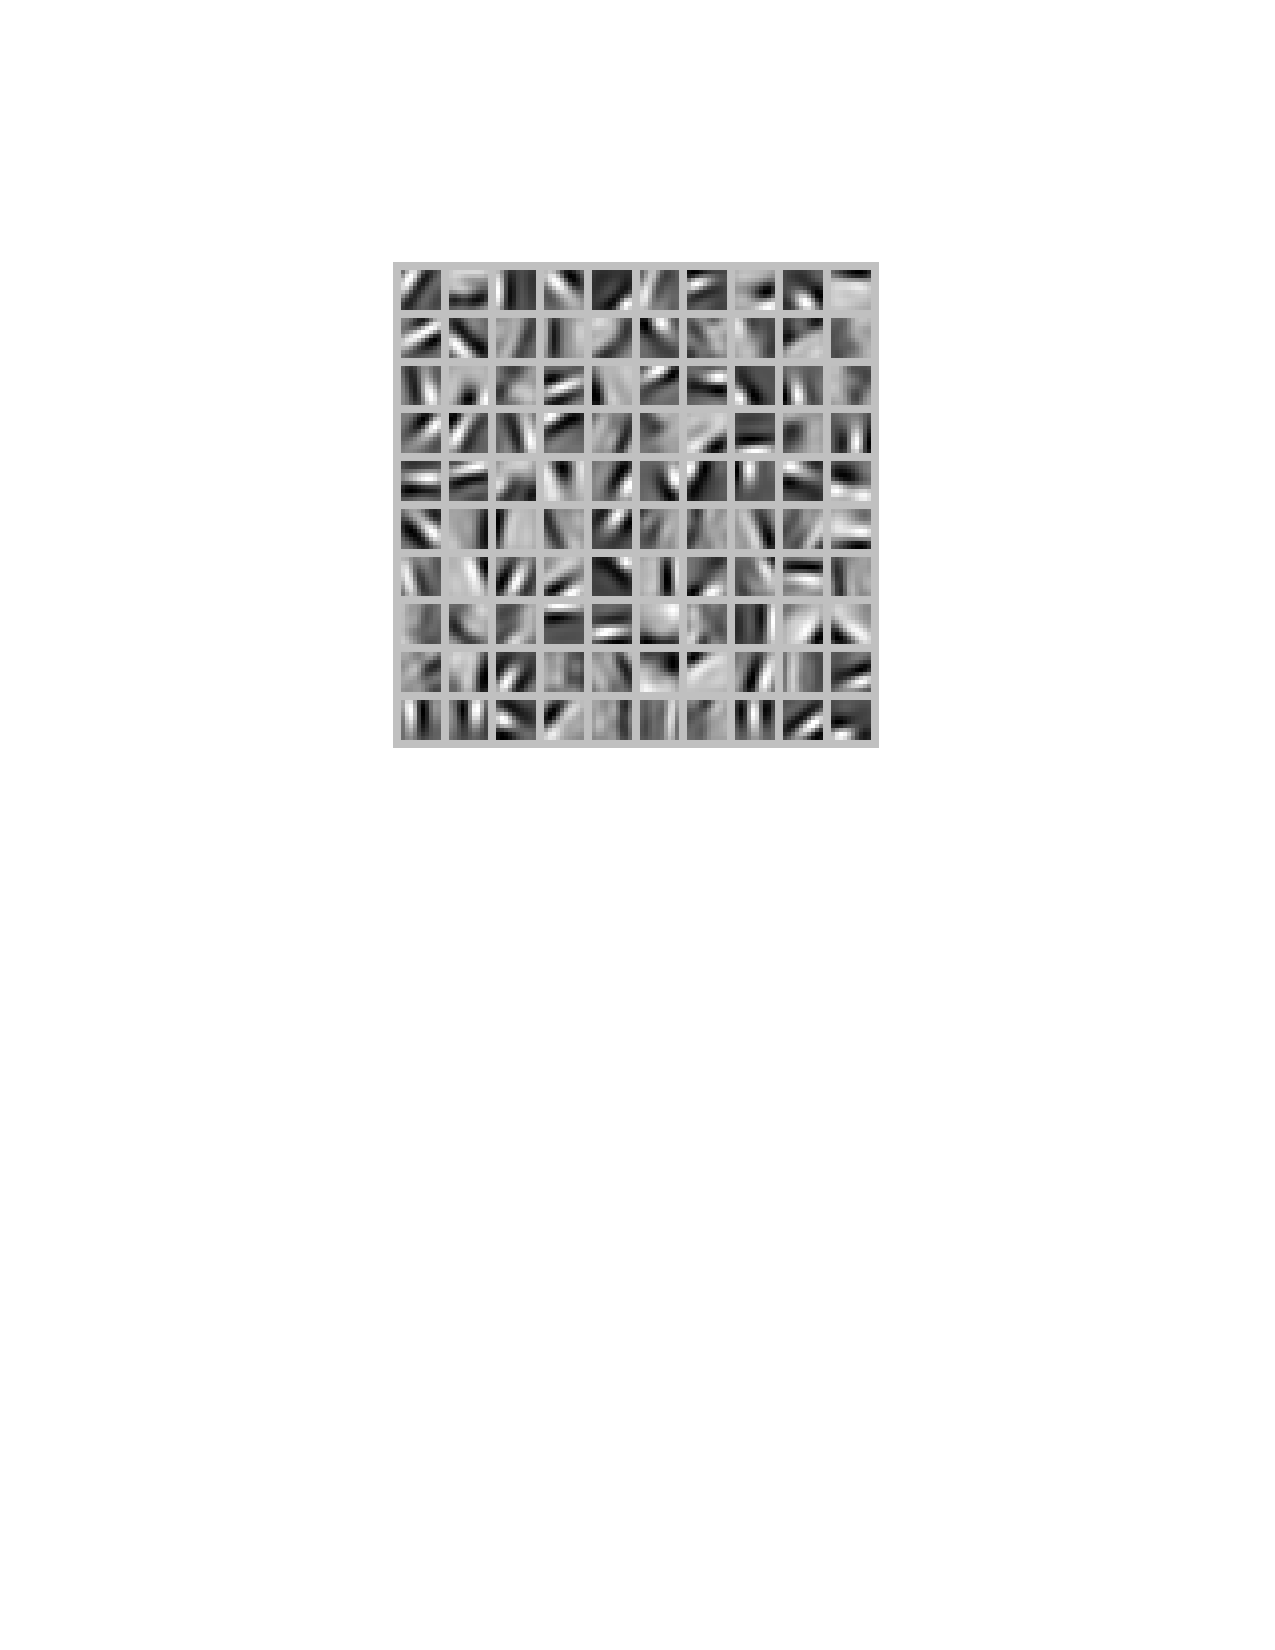
\includegraphics[width=8cm]{fig/1_3.pdf}
\end{figure}

上图的每个小方块都给出了一个(带有有界范数 的)输入图像$ x$ ,它可使这100个隐藏单元中的某一个获得最大激励。我们可以看到,不同的隐藏单元学会了在图像的不同位置和方向进行边缘检测。

显而易见,这些特征对物体识别等计算机视觉任务是十分有用的。若将其用于其他输入域(如音频),该算法也可学到对这些输入域有用的表示或特征。

\section{Summary of notation}
\begin{tabu} to \hsize {|X|X[3,l]|}
\hline

符号 & 含义\nonumber \\ \hline
$x$ & 训练样本的输入特征,$ x \in \Re^{n}$. \nonumber \\ \hline
$y$& 输出值/目标值. 这里 $ y $可以是向量. 在autoencoder中, $y=x$.\nonumber \\ \hline
$(x^{(i)}, y^{(i)})$ &第 $ i$ 个训练样本. \nonumber \\
\hline
$h_{W,b}(x)$&输入为  $x $时的假设输出,其中包含参数 $ W,b$. 该输出应当与目标值 $ y$ 具有相同的维数.
\nonumber \\
\hline
$ W^{(l)}_{ij}$&连接第  $l$ 层 $ j$ 单元和第  $l+1$ 层 $ i $单元的参数.
\nonumber \\
\hline
$b^{(l)}_{i}$&第 $ l+1 $层 $ i $单元的偏置项. 也可以看作是连接第 $ l$ 层偏置单元和第 $ l+1$ 层  $i$ 单元的参数.
\nonumber \\
\hline
$  \theta$&参数向量. 可以认为该向量是通过将参数  $W,b $组合展开为一个长的列向量而得到.
\nonumber \\
\hline
$a^{(l)}_i$&网络中第 $ l $层 $ i $单元的激活(输出)值.
另外,由于$  L_1 $层是输入层,所以 $ a^{(1)}_i = x_i$.
\nonumber \\
\hline
$ f(\cdot)$&激活函数. 本文中我们使用 $ f(z) = \tanh(z)$.
\nonumber \\
\hline
$  z^{(l)}_i$&第 $ l$ 层 $ i $单元所有输入的加权和. 因此有  $a^{(l)}_i = f(z^{(l)}_i)$
\nonumber \\
\hline
$   \alpha$&学习率
\nonumber \\
\hline
$  s_l$&第 $l $层的单元数目(不包含偏置单元).
\nonumber \\
\hline
$  n_l$&网络中的层数. 通常 $ L_1 $层是输入层,$ L_{n_l}$ 层是输出层.
\nonumber \\
\hline
$   \lambda$&权重衰减系数.
\nonumber \\
\hline
$  \hat{x}$&对于一个autoencoder,该符号表示其输出值;亦即输入值 $ x $的重构值. 与 $ h_{W,b}(x)$ 含义相同.
\nonumber \\
\hline
$  \rho$&稀疏值,可以用它指定我们所需的稀疏程度
\nonumber \\
\hline
$   \hat\rho_i$&(sparse autoencoder中)隐藏单元$  i $的平均激活值.
\nonumber \\
\hline
$  \beta$&(sparse autoencoder目标函数中)稀疏值惩罚项的权重.
\nonumber \\
\hline
\end{tabu}

\end{document}